\documentclass[11pt,oneside]{book}
\usepackage[margin=1.2in]{geometry}
\usepackage{setspace}
\usepackage{booktabs}
\usepackage{float}
\usepackage[toc,page]{appendix}
\usepackage[none]{hyphenat}
\usepackage{url}
\usepackage{amsmath}
\usepackage{amssymb}
\usepackage{enumitem}
\usepackage{subcaption}
\usepackage{graphicx}
\usepackage{titlesec}
\usepackage{lipsum}
\titleformat{\chapter}[display]
{\normalfont\huge\bfseries}{\chaptertitlename\ \thechapter}{20pt}{\Huge}
\titlespacing*{\chapter}{0pt}{-50pt}{40pt}
\setlength{\parindent}{0pt}

\begin{document}

\frontmatter

\begin{titlepage}

\begin{center}

\includegraphics[width=5cm]{images/UOSLogo_Portrait_Violet_RGB.png}\\[2cm]
\linespread{1.2}\huge {\bfseries Needle in the haystack: Finding sparse functional status
information with LLMs}\\[2cm]
\linespread{1}
{\Large Alessandro Perelli, Amit Singh, Mahesh Bakal, Molly Senior, Ojas Dudhe, Tara K. Jain}\\[1cm]
{\large \emph{Supervisor:}  Denis Newman-Griffis}\\[1cm]
\large \emph{Report for COM6911} \\[1cm]
May 21st 2025
\end{center}


\end{titlepage}

\newpage

\tableofcontents

\setstretch{1.1} 

\mainmatter

% Executive summary (1 page) — A 1-page summary of the project, to include the main research idea or hypothesis, the main features of the experimental design, a summary of the main result(s), and a conclusion.
\chapter{Executive Summary}
\section{Needle in the Haystack: Investigating Sparse Functional Status Information with NLP}
\subsection{Motivation and Objective}

Functional Status Information (FSI)—which captures a patient's ability to perform daily activities—offers significant potential to enhance clinician insight and support patient-centred care. However, FSI is often embedded within unstructured Electronic Health Record (EHR) notes, making it challenging to systematically identify and extract. This project addresses that challenge by developing and evaluating the use of Natural Language Processing (NLP) models to detect and classify FSI within clinical free-text notes derived from discharge summaries in the MIMIC-IV dataset. The primary objective is to map sentences from the dataset to four key categories based on the International Classification of Functioning (ICF): Mobility, Self-Care and Domestic Life, Interpersonal Interactions and Relationships (IPIR), and Communication and Cognition.

\subsection{Experimental Design and Approach}
Due to the absence of publicly available labelled data for Functional Status Information (FSI) classification, the project adopted two complementary methodological strategies: supervised and unsupervised learning. \medskip

In the supervised learning approach, a silver-standard dataset was manually annotated by the project team, following official ICF guidelines to ensure conceptual alignment with established functional domains. Three models were developed and evaluated for their ability to classify sentences into FSI categories. The first was a CNN-RNN hybrid architecture, which combined pre-trained FastText embeddings with convolutional layers for local pattern extraction and recurrent layers for capturing sequential context. The second was a simpler Feedforward Neural Network (FNN), which operated on mean-pooled FastText embeddings and provided a lower-complexity baseline. The third model was a Random Forest classifier, trained on a hybrid feature set comprising TF-IDF and FastText vectors. Although more interpretable, this model was less capable of capturing the semantic depth and structural nuance of clinical language compared to its neural counterparts. \medskip

The unsupervised learning strategy focused on discovering semantic groupings in the data without the use of annotated labels. Latent Dirichlet Allocation (LDA) was applied to term-frequency-based representations to identify probabilistic topic distributions within the corpus. Additionally, K-Means clustering was used in conjunction with sentence embeddings derived from ClinicalBERT and BioBERT, allowing the grouping of semantically similar sentences based on contextualised representations. A third method involved a hybrid, rule-based approach that leveraged ICF-derived lexicons to assign high-confidence labels to selected sentences, which were then extended through clustering techniques to propagate labels across similar instances. \medskip

\subsection{Main Results}
Amongst the supervised models, a hybrid CNN-RNN achieved the highest performance with a micro-average F1 score of 0.74 - outperforming the fully connected neural network (micro-F1 0.67) and the Random Forest classifier. Sentences pertaining to mobility were identified accurately with a high precision and recall, which may be attributed to a greater abundance of sentences overall for this category in the discharge summaries. The models performed well on sentences related to Communication and Cognition, despite the comparatively limited number of examples in this category.\medskip

Sentences for the IPIR category proved comparatively challenging. It is important to note that due to nuances in its annotation guidelines \cite{InterpersonalGuideline2023}, these were especially complex for manual annotators to identify too. \medskip

The Unsupervised approach with K-Means semantic clustering followed similar trends: it accurately grouped sentences belonging to categories such as mobility and communication, but struggled to isolate the rest. The K-Means clustering with pre-trained Clinical Bert embeddings showed the best performance amongst unsupervised approaches.\medskip

Overall, these findings highlight both the promise and limitations of using NLP techniques for FSI extraction. While high performance was achieved in categories with clearer lexical patterns and more training data, performance can vary substantially across functional domains. This highlights the need for category-specific modelling strategies and improved annotation resources to support more accurate, generalisable and increasingly more nuanced classification.

\subsection{Conclusion and Challenges}
One of the most critical issues was the quality and consistency of manual annotations, particularly across the four ICF categories. Given that annotations were performed by non-experts, variation in interpretation led to label noise that affected the reliability of supervised learning models. Additionally, there was a pronounced class imbalance in the dataset, with Mobility-related sentences overrepresented compared to under-represented domains such as Communication and Cognition. This skew introduced performance bias and limited the models’ ability to generalise across all functional domains. A third challenge lay in the inherent ambiguity of language used to describe functional status; relevant information was often context-dependent or expressed in subtle, implicit ways that were difficult for both human annotators and models to capture.

These limitations underscore the need for a more robust and scalable foundation for future work. In particular, the development of a gold-standard dataset, constructed in collaboration with domain experts, should be prioritised. Such a resource would significantly reduce non-expert label ambiguity and allow for more accurate training, evaluation, and benchmarking of FSI extraction models. \medskip

To address data imbalance and linguistic ambiguity, future work may focus on the exploration of strategies such as data augmentation, semi-supervised learning, and the development of domain-adapted language models suitable for medical use. Techniques like active learning could also improve annotation efficiency and are addressed in greater detail in the discussion and conclusions chapter.\medskip

Despite these challenges, this project demonstrates the feasibility of extracting sparse but clinically valuable FSI from unstructured EHR text. It provides a proof of concept for integrating functional information into computational pipelines and lays the groundwork for more comprehensive, patient-centred data extraction efforts within electronic health record systems. % Ojas 400-500
% Introduction — This section should set the scene for the project, describing the context and ‘big picture’ first, before focusing down on the specific questions that were addressed in the project.

% Comment out the lipsum[1-2] text as you fill in the sections by putting a '%' in front of it.
\chapter{Introduction}

Electronic health records (EHRs) capture large amounts of diagnostic codes, laboratory results and imaging reports. Yet, they still tell us surprisingly little about how patients actually live their lives. 
Decades of studies show that functional status information (FSI) is critical for predicting quality of life, service needs and outcomes such as readmission or mortality. FSI refers to statements that describe what a person can actually do, such as walking to the bathroom unaided or preparing a simple meal. The World Health Organisation's International Classification of Functioning, Disability and Health (ICF) describes functional status as the lived interaction between health conditions, body structures, activities, participation and contextual factors, showing its centrality to truly patient-centred care. By focusing on whole-person performance rather than isolated impairments, FSI offers a genuinely patient-centred lens on health and doesn't just focus on whether the heart is functioning or a lab value is normal for example, but whether the individual can return to work, live independently and engage meaningfully with family and society. \\

Unfortunately, FSI is a needle in the clinical-text haystack. It is buried in narrative notes and expressed with highly variable language ("walks with a stick", "mobilised 20m independently" etc.). The absence of publicly available, labelled corpora has left traditional NLP approaches ineffective, which has constrained progress in this area of health informatics. Recent annotation projects have begun to define strict guidelines for the following categories:

\begin{itemize}
    \item Mobility - this includes things like moving the whole body from place to place (walking, climbing stairs, getting in and out of a car etc.) It also refers to the use of mobility aids (canes, walkers, wheelchairs etc.).
    \item Self-care and Domestic Life (SC/DL) - this includes personal activities of daily living (ADLs) such as bathing, dressing, eating etc. It also includes instrumental tasks (such as cooking, cleaning, shopping etc.) and safety and environmental management (using kitchen appliances, handling emergencies at home etc.).
    \item Interpersonal Interactions and Relationships (IPIR) - this includes initiating and sustaining relationships (such as family roles, friendships intimate partnerships etc.). It also involved cooperating with others in shared activities (coordinating appointments, caregiving, teamwork etc.) and social behaviours and norms (expressing emotions appropriately, resolving conflict, seeking assistance etc.)
    \item Communication and Cognition (Com/Cog) - this includes receptive and expression communication (like understanding spoken or written language, speaking clearly, writing and using assistive communication devices). It also contains higher cognitive functions (like memory, orientation, planning etc.) and conversation skills (like taking turns, staying on topic, using non-verbal cues etc.).
\end{itemize}

Using different NLP approaches, our project aims to automatically classify sentences from free-text clinical notes (from the MIMIC-IV dataset) into the four ICF activity domains. We have identified this task as a multi-label, multi-class sentence classification problem, where each sentence can belong to one or more of the categories mentioned by the ICF. \\

To support supervised learning, we manually annotated a representative subset of MIMIC-IV discharge summaries by hand, creating a silver standard. We could not use the gold standard created in the paper "Inductive identification of functional status information and establishing a gold
standard corpus" \cite{thieu2017} due to it not being publicly released yet (something which seems less and less likely due to the ongoing academic situation in the US) and therefore had to manually annotate this data ourselves. \\

Having established this silver standard, we pursued two modelling approaches. Unsupervised learning was useful because a large, expertly annotated gold standard simply does not exist for function status (or at least, not a public one as mentioned before). Therefore, letting the data organise itself exposes the latent themes that recur across notes without requiring clinicians to label every sentence. Such themes can be modelled either:

\begin{itemize}
    \item Probabilistically - with term-frequency Latent Dirichlet Allocation (LDA)
    \item Geometrically - by clustering dense semantic embeddings from a language model such as ClinicalBERT.
\end{itemize}

In practice, the embedding-based clusters capture functional nuance far better than the bag-of-words topics. Unsupervised approaches can effectively provide a subset from a larger dataset and work as a sieve for annotators looking to create a labelled dataset to train a supervised model on. \\

In comparison, supervised learning is the natural choice once a dataset has been labelled because the task then becomes multi-label topic classification, that is given a sentence, decide which ICF domains it conveys. Yet this is still far from trivial. Functional status language is notoriously varied and complex. With ambiguous sentences and cryptic abbreviations, a model must generalise effectively across all this. Sophisticated architectures must be implemented in order to fully capture meaning, as well as a high volume of accurately manually annotated data. Where those hurdles are overcome, supervised learning provides the precise and dependable decision boundaries needed for accurate and reliable classification. \\

The next chapter looks at the existing literature on extracting functional status information from clinical text. Particular attention is paid to why capturing function in health is so important, the current dataset annotation and pre-trained embeddings and current work on supervised and unsupervised models for this task. % Alessandro 1000
% This section will briefly cover the technical background to the project, and review the relevant literature. The literature review should critically assess recent and relevant papers, identifying gaps in knowledge, and linking to the project. You may wish to compare (identify similarities) and contrast (identify differences) as part of this process, as well as highlighting clear limitations associated with some papers in the literature. This section should culminate in the rationale for your project. 

% What has been done on NLP analysis of FSI in the past, and how you have drawn from this literature for your project.

% Comment out the lipsum[1-2] text as you fill in the sections by putting a '%' in front of it.

\chapter{Background and Literature Review}

\section{Introduction}

Though the topic of capturing FSI from EHRs is of great importance, the previous research carried out in this area is not extensive. The search for literature involved identifying the necessary methodological steps that must be carried out in this research project and searching for literature accordingly. Keywords and phrases included: FSI, disability, EHR, sentence classification, MIMIC, clinical notes, ICF, NLP, and more. \\

This literature review has been structured by methodology, split into the two main approaches taken, supervised and unsupervised techniques. It will then outline the background of this topic, annotation of the dataset, any important decisions regarding pre-processing steps, and finally, suggested models for this problem and problems of a similar nature in order to guide the pipeline used in this research project.

\section{Background}

\subsection{The case for capturing function in health}

There is a compelling case to be made regarding the treatment of functional status as a primary data element and not just an afterthought. The paper "Broadening horizons: The case for capturing function and the role of health informatics in its use" \cite{newman-griffis2019bh} explores how, because functional outcomes reflect the cumulative impact of multiple conditions, they overcome the fragmentation caused by disease-specific metrics and correlate strongly with quality of life, resource needs and even mortality risk. The paper shows that even though most of this information already exists in free-text notes, it remains invisible to analytics. Therefore, modern informatics (especially NLP that mines narrative EHRs) can surface and standardise this data with little extra effort from clinicians. To achieve this goal, four steps were proposed:

\begin{itemize}
    \item Publish shared annotation standards and datasets
    \item Frame common NLP tasks
    \item Build a machine-readable ontology linking ICF concepts to clinical vocabularies
    \item Embed routine documentation triggers in care workflows
\end{itemize}

Overall, this paper provides both the rationale and a practical roadmap for integrating functional status into population health monitoring. It provides clear reasons as to why developing such systems is so important.

\section{Supervised Techniques in Natural Language Processing}

\subsection{Dataset annotation}

Thieu et al. \cite{thieu2017} proposed an approach to identify and structure functional status information (FSI) specific to the domain of mobility off the International Classification of Functioning, Disability, and Health (ICF) from free-text clinical records. Utilizing over 1,200 physical therapy notes from NIH Clinical Centre, the authors designed an annotation framework, distinguishing Action, Assistance, Quantification, and Score Definition. Their methodology got a curated gold-standard corpus consisting of 250 annotated notes, achieving an average F1 score of 97\% for textual span overlaps, and kappa scores ranging from 0.4 to 0.9 for attribute-level annotations. The manual annotation process is described as labour-intensive; this resource provides a foundation for future NLP-driven extraction and analysis of FSI, and demonstrates potential applicability beyond mobility to other domains within the ICF framework. \\

On the other hand, to directly address the problem of having no publicly available annotated dataset, Le et al. \cite{le2023} aimed to use deep active learning to construct a gold standard annotated corpus for the mobility domain of the ICF in order to facilitate the automatic extraction and analysis of FSI in free-text clinical notes. Using the n2c2 dataset, they implemented active learning through query-by-committee sampling (using BERT and CRF models) to select the most informative sentences for human annotation. The gold-standard dataset produced was then used to retrain their mobility NER model using a variety of BERT pre-trained embeddings. An F1 score for each entity was produced, with a score of around 0.83 for the action entity in all models tested. This paper is constrained by its focus on mobility, only one of four domains from the ICF, limiting broader applicability to the other ICF categories; however, it provides justification for selecting only to look at the action entity since this is the most indicative for identifying mobility statements.

\subsection{Pre-trained embeddings}

Newman-Griffis et al. \cite{newman-griffis2019hare} introduced HARE, a system designed to highlight relevant information in clinical narratives using fast token-level relevance tagging and document ranking. In the model they used both static (FastText) and contextual embeddings like ELMo and BERT to extract features for each token and applied a feedforward neural network for classification. To refine the output, they implemented post-processing techniques such as threshold tuning, collapsing adjacent segments, and Viterbi smoothing. They found that FastText resulted in the best F-Score with BERT contextualised embeddings close behind. The insights provided in this paper about the different sorts of embeddings will be crucial for constructing our pipelines, with an emphasis on speed, interpretability and effective handling of imbalanced data in HARE providing strong support for the design and functionality of our model.

\subsection{Supervised models}

Extracting valuable information from EHRs is a problem faced by many researchers, Houssein et al. \cite{houssein2023} aimed to automatically detect 11 cardiovascular risk factors and their temporal attributes from free-text clinical notes using a stacked-embeddings deep-learning approach. They stacked BioClinical BERT embeddings with Character BERT and ran a single-layer RNN over the stacked embeddings to produce an F1 score of 93.66\% which outperformed the conditional random field (CRF) baseline previously thought to be the most advanced technique for information extraction. This method relies on having a large sample of annotated records, with no provisions for a low-resource adaptation. This research also focuses on extracting cardiovascular risk factors, not FSI information; however, as the task is of a similar nature to this project, it is still very relevant. Due to the time constraints of this project, the light-weight architecture employed in their paper provides grounding for a light-weight model to be used in this project. \\

With a problem more similar to our own, Newman-Griffis \& Fosler-Lussier’s paper \cite{newman-griffis2020auto} aims to demonstrate that a weakly-supervised guideline-driven pipeline can effectively train a feed-forward neural network to map free-text sentences in clinical corpora to ICF codes, without requiring hand-annotated datasets. They found that the FNN trained on silver-labelled sentences from the mobility domain achieved a micro F1 score of 0.74 substantially outperforming both rule-based and classical ML baseline models (SVM, random forest). They theorised that although the model was tested on the mobility domain, the same model could be applied to the other ICF domains. Though the feed-forward network performed the best out of the tested models, it may have struggled to learn more complex patterns or relationships that a CNN, RNN or Transformer could model. The problem set out in this paper is slightly different from the problem faced in our research however, this paper still provides support for the implementation of a FNN model for our problem and the potential for extension to a deeper neural network that could further improve the F1 score.

\section{Unsupervised Techniques in Natural Language Processing}

\subsection{Latent Dirichlet Allocation (LDA)}

Latent Dirichlet Allocation (LDA), a probabilistic generative model introduced by Blei et al. \cite{blei2003}, has become a foundational technique for uncovering latent semantic structures in large-scale textual datasets. Its ability to model documents as mixtures of latent topics, each represented as distributions over words, makes it particularly well-suited for analyzing unstructured clinical narratives, such as those found in the MIMIC-IV database. \\

LDA has been widely applied in various domains, including digital health and mental health informatics, where it facilitates the extraction of thematic patterns from user-generated content. For example, Low et al. \cite{low2020} utilized LDA to identify emerging discourse trends in digital mental health support groups during the COVID-19 pandemic. These applications demonstrate LDA’s effectiveness in extracting latent structure from noisy, health-related text—a task analogous to modelling the complex linguistic features of discharge summaries. \\

In the clinical context, discharge summaries provide rich, narrative records and are written by healthcare providers to document diagnoses, treatments, clinical decisions, and patient outcomes. However, the lack of explicit structure and annotation in these texts poses challenges for large-scale information extraction and downstream classification. LDA offers a potential solution by clustering documents based on thematic similarity, which can serve as a preliminary step in annotation pipelines. \\

Note that while LDA is a powerful tool for uncovering latent topics in raw textual data, it operates under assumptions that are incompatible with the nature of ClinicalBERT embeddings. \\

LDA requires input in the form of discrete term-document frequency matrices, such as bag-of-words or TF-IDF representations, where each document is a probabilistic mixture of topics, and each topic is a distribution over words. This framework is well-suited for count-based, sparse data.

\subsection{K-Means clustering}
The integration of transformer-based models with clustering algorithms has significantly advanced the analysis of unstructured clinical text. ClinicalBERT, a domain-specific adaptation of BERT fine-tuned on clinical notes, captures the nuanced language of medical documentation more effectively than general purpose models. \\

When ClinicalBERT embeddings are subjected to K-Means clustering, they facilitate the grouping of semantically similar discharge summaries, unveiling latent structures and common themes within the data. A notable study by Huang et al. \cite{huang2019} utilized ClinicalBERT to model clinical notes and predict hospital readmissions, showcasing the model's capability in understanding complex clinical language. \\

In order to facilitate this second clustering approach a hybrid methodology to label FSI categories from clinical sentences, starting with a rule-based system, its structure put together from official ICF documentation \cite{CommCognitionGuideline2023, InterpersonalGuideline2023, MobilityGuideline2023, SelfCareGuideline2023}. Parallel to previous work using lexicon-based methods, this method involves creating dictionaries consisting of domain-specific phrases and keywords for each ICF domain and applying rules to ascertain relevant mentions. As described by Zheng et al. \cite{zheng2010} and executed in tools like ClinicalRegex, rule-based systems allow for clear and high interpretability, strict command over parameters, and transparency of decision making, which is of much value in clinical practice. Although such methods can struggle with range and exceptional cases, their reliability in high-confidence settings accounts for their use in early labelling \cite{hong2020}. \\

To take this labelling process further and generalize the model beyond surface keywords matching, the implementation of a second component involving unsupervised clustering was considered. One of the proposed methods was to use K-Means clustering over clinically contextual sentence embeddings generated from a domain-specific BioBERT Model. This semi-supervised auto-labeling approach was derived from previous work such \cite{eisman2021, greenes2018}, who presented that layering rule-based with clustering and propagation can effectively vary range of labeled datasets in low-source clinical settings.  This strategy uses the semantic generalization of contextual embeddings with high efficiency of Rule-based methods, forming a middle-ground between accuracy and interpretability in early-set ICF annotation systems.

\section{Conclusion}

Overall, the literature set out above has demonstrated that FSI can be extracted from EHRs using a variety of NLP approaches. Often opting for simple feed-forward or rule-based pipelines, the previous research achieves respectable results, though often discarding word-order or syntactic information. This is something that deeper architectures, such as CNNs or RNNs, have shown promise in, but have yet to be applied to a multi-label FSI extraction problem. \\

The majority of the papers focused solely on the mobility domain of the ICF framework, with no empirical testing on the other three domains, likely due to the abundance of mobility-related terms in the dataset with easily distinguishable keywords such as “walk”. The more complex language and relationships in the other domains pose a challenge to research done in this area, however, it is something that our project aims to address and will be a key focus going forward. \\

Another key issue across the majority of the papers is the availability of a gold-standard labelled dataset from any of the accessible free-text clinical databases. Though this is not the focus of our research, it is a problem that will need to be considered when creating our model. \\

In conclusion, though limited, the literature provides a rich methodological framework that can help guide our research and our model pipeline. Because of the complexity of the problem of FSI extraction, it can be framed in many different ways. How we approach the problem set out in our initial objective will be a key factor in determining how well we are able to get our model to perform and the outcomes and insights we will be able to extract.
 % Molly 2000
% This is a duplicate research-question section that can be used as is and incorporated into the report.
% A short section which summarises the hypothesis or research question(s) that is addressed in the report. This should be a logical development of the preceding section, and may include a list of concrete objectives for the project.
% Link back to the original proposal posed by Denis.
% Lead in from literature review and link to methodology (next section).

\chapter{Research Question}
\section{Problem Landscape and the Role of NLP}

In this project, we set out to investigate the feasibility of NLP models and techniques for the extraction of Functional Status Information (FSI) from free-text clinical records. As discussed in the previous section, functional status is a primary data element that offers valuable insights to clinicians. While essential for understanding the lived experience of health, its extraction is highly complex due to its inconsistent expression and sparse representation in discharge summaries. \medskip

No publicly available FSI datasets currently exist, adding significant complexity to the use of supervised machine learning techniques. Although detailed annotation guidelines have been developed for several functional status domains—most notably Mobility \cite{nih_mobility_guideline}—the sensitive nature of the MIMIC-IV dataset prohibits the direct use of mainstream large language models (LLMs) for this task. For instance, it is not permissible to upload this data to commercially hosted LLM APIs. Nevertheless, the publication of such guidelines by institutions like the NIH reflects a growing recognition among clinicians and healthcare researchers of the potential for NLP techniques to address this challenge.\medskip

Given these constraints, researchers have begun exploring alternative methodologies that leverage recent advances in NLP while maintaining stringent data privacy protocols and regulatory compliance \cite{kumar2024gpt}. Our \textbf{primary objective} is to assess the feasibility of designing a bespoke technical infrastructure to extract, annotate, and ultimately classify FSI—with increasing precision and nuance—from unstructured clinical narratives.

\section{Feasibility of Leveraging Sparse FSI in a clinical dataset for NLP models}
\medskip
The project explores whether a small, manually annotated subset of clinical free-text sentences can serve as a sufficient foundation for training reliable models to classify Functional Status Information (FSI) into the appropriate ICF categories.\medskip

This study also examines the limitations and challenges posed by the semantic sparsity and contextual ambiguity of FSI data in real-world clinical notes, and how these factors may impact the generalisability and performance of the models developed. These concerns are addressed in further detail in the Discussion section.
\medskip
\section{Assessing different Modeling Approaches for FSI Classification}

We aim to investigate the relative strengths, feasibility, and limitations of multiple modelling paradigms—including unsupervised clustering methods, rule-based heuristics, and supervised neural network models.\medskip

Our analysis also explores the differential performance of models across the four ICF domains, identifying contributing factors such as vocabulary range, domain-specific semantic overlap, and class imbalance, and how these influence overall classification outcomes.\medskip

In parallel, we pursue a methodological objective: to evaluate the practical effectiveness of recent advancements in NLP, such as the use of ClinicalBERT embeddings in scalable clustering models run on high-performance computing (HPC) systems, and the integration of pre-trained FastText embeddings within a CNN-RNN architecture for multi-label classification. The following section outlines the methodologies employed in our investigation in greater detail.

\medskip
In summary, this study seeks to answer the following research questions:

\begin{enumerate}
\item Can foundational NLP techniques and models be leveraged to design a system for extracting and classifying Functional Status Information from unstructured clinical text?
\item What are the relative strengths and limitations of different approaches in NLP? Specifically, how do supervised and unsupervised methods differ in their performance, and how do the strengths of different models in each approach guide model selection in this context?
\end{enumerate}

The following section outlines the methodologies employed in our investigations in greater detail.

 % Ojas 300 - 500 [Denis,"focus on the end game, rather than the initial direction."]
% In this section you should describe what you have done in sufficient detail to enable another research or team to repeat your study. Depending on your project, you will need to include a description of and justification for the experimental design, code development, details of data analysis, and production of results. Some details of the methods could be included in an Appendix.

\chapter{Methodology}

\section{Dataset}
This project utilizes the MIMIC-IV dataset \cite{mimiciv} which is a publicly available, de-identified database of patient records from the Beth Israel Deaconess Medical Center, covering ICU admissions between 2008 and 2019. We utilized the discharge summaries made available through this dataset which provide functional status information of patients in free-text notes. \\

The subset used for analysis comprises approximately 3.28 GB of unstructured clinical text. These summaries were chosen for their richness and relevance to both unsupervised and supervised learning tasks.\\

Access to the data was obtained via the PhysioNet credentialing process, which involves completing data usage training and agreeing to ethical use guidelines. 


\section{Pre-processing}
The text preprocessing pipeline includes the following steps:

\begin{itemize}
    \item \textbf{Sentence Segmentation:} Raw clinical texts (discharge summaries from the \texttt{discharge.csv} file in the MIMIC-IV dataset) are segmented into individual sentences using the spaCy NLP library, which applies rule-based syntactic parsing to identify sentence boundaries.

    \item \textbf{Text Preprocessing:} Sentences are cleaned by removing markdown syntax, list indicators, and excess whitespaces to reduce noise and standardize formatting.

    \item \textbf{Filtering:} Sentences that are too short, purely numeric, or lack alphabetic characters are excluded to retain only linguistically and semantically meaningful entries.
\end{itemize}

The cleaned sentences are compiled into a structured tabular format, suitable for downstream machine learning tasks and manual annotation workflows for both supervised and unsupervised models.

 
\section{Design of Unsupervised Models}

\subsection{LDA with TF and K-Means with ClinicalBERT}

To retain semantic meaning in clustering discharge summary sentences, two approaches were used:

\begin{itemize}
    \item \textbf{Term Frequency with LDA:} LDA was applied to term frequency vectors to identify interpretable clinical topics based on word co-occurrence. This method captures the broader thematic structure in the text.
    
    \item \textbf{K-Means with ClinicalBERT:} ClinicalBERT embeddings provide context-aware representations tailored to medical language. Applying K-Means to these embeddings enables unsupervised grouping of semantically similar sentences, even when they differ in wording. ClinicalBERT was selected for its domain-specific training on clinical notes, thereby making clusters based on the semantic relevance of text-processed tokens.
\end{itemize}

Using both methodologies provides complementary perspectives, LDA captures latent topic structures through word co-occurrence patterns, while the ClinicalBERT with K-Means clustering captures semantic similarity using contextual embeddings. This dual approach allows for a comparative analysis of clustering quality and interpretability. Both of these approaches were implemented with scalable python frameworks such as PySpark to enable the algorithms to run on High Performance Computing (HPC)\footnote{The relevant code for scalable clustering models can be found here: \url{https://github.com/twinzies/fsi-nlp} and also at \url{https://github.com/AlessandroPerelli/com6911-teamdn1/tree/main/unsupervised_model/fsi-nlp} This complements the code that can be run on limited computational resources such as a PC: \url{https://github.com/AlessandroPerelli/com6911-teamdn1/tree/main/unsupervised_model/kmeans-ClinicalBERT}} \medskip


In the LDA approach, bag-of-words and term frequency representations were used to generate topic distributions. For the K-Means approach, word-level embeddings were generated using ClinicalBERT. These embeddings enabled the clustering of semantically similar sentences. Both methods were compared with traditional feature extraction techniques to evaluate their effectiveness. The probabilistic formulation of LDA is given by the following generative process.

\begin{align*}
\theta_d &\sim \text{Dirichlet}(\alpha) \quad \text{(document-topic distribution)} \\
z_{dn} &\sim \text{Multinomial}(\theta_d) \quad \text{(topic assignment)} \\
w_{dn} &\sim \text{Multinomial}(\beta_{z_{dn}}) \quad \text{(term from topic)}
\end{align*}

The joint probability models the generative process of the documents, enabling the discovery of latent semantic structures based on term frequency inputs. This formulation is expected to allow the LDA approach to effectively uncover underlying topic patterns across the corpus. The joint probability is given by:
\[
P(\theta, z, w \mid \alpha, \beta) = \prod_{d=1}^{D} P(\theta_d \mid \alpha) \prod_{n=1}^{N_d} P(z_{dn} \mid \theta_d) P(w_{dn} \mid z_{dn}, \beta)
\]

Where,
$w_{dn}$ = term frequency (TF) of the $n$-th word in document $d$, 
$z_{dn}$ = topic assigned to word $w_{dn}$, 
$\theta_d$ = topic distribution for document $d$, 
$\beta$ = topic-word distribution, 
$\alpha$ = Dirichlet prior for $\theta$. \bigskip

In this formulation, $K$, the number of topics, determines the dimensionality of the document-topic distribution $\theta_d$, the set of possible topic assignments $z_{dn}$, and the size of the topic-word distribution matrix $\beta$. Though not explicitly shown in the equations, $K$ governs the latent structure over which the LDA model is defined.\bigskip

KMeans clustering, applied to ClinicalBERT embeddings, is formalized by the following objective function.

\[
\underset{C}{\arg\min} \sum_{i=1}^{k} \sum_{x \in C_i} \| x - \mu_i \|^2
\]

Where, 
$x$ = ClinicalBERT embedding of the tokens of the document, 
$k$ = number of clusters, 
$C_i$ = set of points assigned to cluster $i$, 
$\mu_i$ = centroid of cluster $i$, computed as:
\[
\mu_i = \frac{1}{|C_i|} \sum_{x_j \in C_i} x_j
\]


\subsection{Rule Based with K-Means}

\begin{itemize}
    \item Rule-based labelling: Part A of Hybrid model consisting of preprocessing, which includes lowercasing, punctuation removal, tokenization, and lemmatization using NLTK. Initially, sentences were matched against manually crafted keywords and phrase dictionaries consisting of 4-ICF aligned categories. Each dictionary consists of around 30 keywords and domain-specific phrases. A sentence was given a Rule-based label if it matched at least one phrase or keyword. This resulted in high precision initial labelling, with keeping unlabeled sentences untouched. 
    \item BioBERT with k-means: Further in Part B of Hybrid model, Sentences embeddings were created using BioBERT model with a 768-dimensional output. K Means clustering was used with k=10, n\_init=10 over the group of around 50,000 sentences based on semantic similarity. For each cluster, label purity was measured based on the existing Rule-based labels. If the dominant label accounted for more than 80\% of the labelled sentences in that particular cluster, and the cluster size was more than n=30, the label was propagated to all the previously unlabeled sentences within that cluster that had a token count of at least 5, to remove any accidental labellings. \\
\end{itemize}
This two-staged hybrid approach enabled both high-confidence initial annotation through manually derived rules and broader semantic generalization through unsupervised clustering. While the approach was highly effective and did as expected in capturing structured FSI- related content– particularly in categories such as Mobility and Communication \& Cognition, which presented higher precision – manual inspection revealed challenges and difficulties faced by the model in categories like IPIR and SC/DL, where key-word based rules and embedding similarity often struggled with contextual ambiguity. Nevertheless, the combination of rule-based and clustering based components provided a flexible, interpretable framework for early-stage annotation of FSI statements in low-resource settings

 
\section{Design of Supervised Models}

\subsection{Annotations}

In order to develop supervised models, we needed to manually annotate our data as mentioned before. To do this, we divided the data (around 44000 lines) between five team members. After labels were assigned with reference to the ICF annotation guidelines \cite{CommCognitionGuideline2023} \cite{MobilityGuideline2023} \cite{InterpersonalGuideline2023}, the team cross-validated the labeling and annotation efforts. Then the splits were combined to form various datasets for experimentation and model development:

\begin{itemize}
    \item Full dataset - contains every annotated sentence, including all 0 labels.
    \item Label dataset - contains every annotated sentence, excluding all 0 labels.
    \item Category-specific datasets - four separate files, one for each ICF category, each containing all sentences that carry that label (and only that label).
    \item Multi-label only dataset - this dataset contains all the sentences which have two or more labels.
\end{itemize}

\subsection{CNN-RNN}

One of the models implemented was a CNN-RNN hybrid model. This model uses pre-trained FastText embeddings, a convolutional layer with ReLU activation and adaptive max-pooling, a recurrent layer, specifically GRU, is used as it is more lightweight than LSTM, a dropout layer to mitigate overfitting, and a fully-connected output layer. Finally, this model makes its multi-label predictions using a sigmoid activation function that produces independent probabilities for each label with a decision threshold of 0.5 for each class assignment, allowing the model to assign multiple labels to a singular sentence. Binary cross-entropy loss is applied to all four labels, and an Adam optimiser is implemented. Early stopping is also used with a patience of 3 in order to stop over-fitting in the model. Though this is a reasonably lightweight model, the negative samples (sentences labelled 0) were undersampled by 95\% in order to create a more even split between the positive and negative sentences and cut down on training time. A stratified split was used to create train, test and validation sets to ensure an even split of all four labels. Fig.~\ref{fig:cnn-rnn-arch} shows a diagram of the model's architecture. \\

\begin{figure}
    \centering
    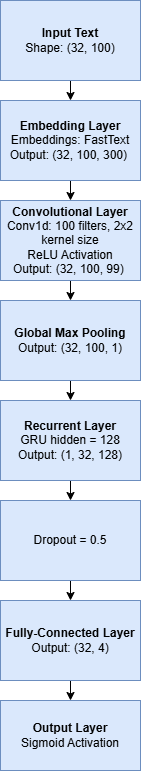
\includegraphics[width=0.1\linewidth]{myReport/figures/CNN-RNN.drawio.png}
    \caption{CNN-RNN Hybrid Model Architecture}
    \label{fig:cnn-rnn-arch}
\end{figure}

 
\subsection{FNN}
Another model we explored was an FNN. FNN's are commonly used for NLP tasks, so this model is not only suitable for this task, but provides for a good comparison with the CNN-RNN hybrid model. This FNN relies on a simple bag-of-embeddings representation of each sentence. All tokens are first projected into 300-dimensional pre-trained FastText vectors (the same used in the CNN-RNN hybrid model). Padding tokens are masked out and the remaining embeddings are mean-pooled to give a single, fixed-length sentence vector. \\

This vector is then passed through two fully connected hidden layers of 256 and 128 units, each followed by a ReLU activation and a 0.5 dropout layer to reduce over-fitting. A final linear layer with sigmoid activation produces four independent probabilities, one for each ICF category and a decision threshold of 0.5 converts these probabilities into binary labels, allowing multiple categories to be assigned simultaneously. Training follows the same procedure used for the CNN-RNN hybrid model for ease of comparison. This is:

\begin{itemize}
    \item Vocabulary is capped at 1000 tokens and sentences are truncated/padded to 100 tokens.
    \item The dominant “no-label” samples (category 0) are under-sampled by 95\% to balance the four positive classes and reduce training time.
    \item A 64/16/20 split is used for train, validation and test sets to preserve label distribution.
    \item Optimisation uses binary cross-entropy loss, the Adam optimiser ( with a learning rate of 0.001 and a batch size of 32) and early stopping with a patience of 3 based on validation micro-F1.
    \item Embedding weights (except the padding vector) are fine-tuned during training, keeping the model lightweight and computationally efficient.
\end{itemize}

\subsection{Random Forest}
The final model we implemented is a Random Forest classifier using a hybrid model that combines TF-IDF and FastText embeddings to classify clinical sentences into functional status categories. TF- IDF captured the most important words from the text while FastText provided a deeper meaning by focusing on each word and turning it into a dense vector using pre-trained vector embeddings. These two features were then combined to give the model both lexical and semantic information. The classifier was then set up to handle multi-labels classification which means that it could assign more than one label like Mobility, Self-care and Domestic life, Interpersonal Interactions and Relationships, Communication and Cognition to each of the sentences. We used 100 trees in the forest and set a maximum depth of 20 to balance accuracy and efficiency. Since the test data was not labeled, we evaluated the model on training data using precision, recall and F1-score and then visualized the results using a bar chart. We have also plotted how many times each label is  predicted in the test set and also printed 30 predicted sentences to see how our model performed. While the model worked well with Mobility related information, it struggled with less common categories due to the class imbalance and the lack of more advanced techniques like class weighting or sampling. Still, this method was fast, interpretable, and useful as a starting point for functional status classification\footnote{The relevant code for supervised models can be found here \url{https://github.com/AlessandroPerelli/com6911-teamdn1/tree/main/supervised_model}.}. \medskip


\section{Evaluation}

% Evaluated with micro-F1 because of the imbalanced classes. 
\subsection{Unsupervised Models}

Due to the lack of reliable ground truth labels for most of the dataset, we evaluate unsupervised models using a combination of cluster performance metrics—such as silhouette scores and perplexity—and qualitative methods including visual inspection and topic exploration through word clouds. All unsupervised algorithms are developed using PySpark to ensure scalability and are executed on a high-performance computing (HPC) environment to efficiently process large volumes of text data.\medskip

While evaluation metrics such as Gini Impurity Index and accuracy were initially considered to assess cluster purity and classification performance, they were ultimately deemed unsuitable for this approach of the study. The primary reason was the limited reliability of the categorical labels used for evaluation, which were assigned without clinical expertise and exhibited inconsistencies upon cross-validation.

\subsubsection{Scalable ClinicalBERT with K-Means Clustering}

We generate sentence embeddings using ClinicalBERT and apply K-Means clustering to group semantically similar content. We assess cluster quality using silhouette scores, which quantify how well each sentence fits within its assigned cluster relative to others. To support visual interpretation, we use dimensionality reduction techniques such as t-SNE and PCA, enabling 3D visualizations of the clustering structure. For interpretability, we construct word clouds based on the most frequent terms within each cluster to highlight the dominant themes.\medskip

\subsubsection{Scalable LDA with Term Frequency}

We implement Latent Dirichlet Allocation (LDA) on tokenized text data, following preprocessing steps including stemming, lemmatization, and stop word removal. Since LDA operates on term frequency rather than contextual embeddings, we use raw term counts as input. We evaluate model performance using perplexity scores, where lower values indicate better generalization. Additionally, we manually review the top words within each topic to assess semantic coherence and thematic relevance.

\subsubsection{Rule-Based with K-Means Approach}

Without ground truth labels, we evaluated our rule-based K-Means method using internal metrics and manual review. We assigned initial labels using handcrafted keyword dictionaries for four ICF categories, then generated BioBERT embeddings for sentence representations. Using K-Means ($k=10$), we clustered semantically similar sentences. We propagated labels within high-purity clusters (defined as those with more than 80\% of sentences sharing the same rule-based label and at least 30 samples). \\

For visualization, we reduced dimensions with UMAP to inspect cluster distribution against functional categories. Manual review confirmed strong performance for Mobility and Communication \& Cognition categories, with less consistency in ambiguous categories like Interpersonal Interactions \& Relationships and Self-care \& Domestic Life The hybrid approach effectively expanded our labeled dataset semi-automatically while maintaining interpretability and resource efficiency.


\subsection{Supervised Models}

We evaluated our supervised models using standard multi-label metrics: \textbf{precision}, \textbf{recall}, and \textbf{F1-score} (micro and macro averages). Accuracy is not a suitable metric for this problem due to the imbalanced classes in the dataset and therefore was not used for evaluation. Data was split 64\%/16\%/20\% (train/validation/test) with stratification to maintain label balance. A confusion matrix and learning curves for each of the neural models was also produced. \\

The \textbf{CNN-RNN} model performed best overall, especially for well-performing categories like Mobility and Communication \& Cognition. Our \textbf{FNN} model was lighter and faster while remaining competitive. Both neural models used validation micro-F1 for early stopping to prevent overfitting.\\

Our \textbf{Random Forest} model, which used combined TF-IDF and FastText features, performed adequately for frequent labels but struggled with class imbalance and lacked the expressiveness of deep models. Without a proper test set, Random Forest evaluation relied on training data and qualitative assessment.
 % Amit 1500 - 2000
% In this section you should present the results and main findings from your project.
\chapter{Results}

This chapter presents the final results from the supervised and unsupervised model methods applied in the project. Detailed results, including visualizations and tables, are provided for clarity.

\section{Unsupervised models}

\subsection{Scalable clustering models}

Topic modeling using LDA was used for sentence embeddings to discover latent patterns in the data. Additionally, semantic clusters were made with K-Means clustering on ClinicalBERT embeddings of the data. Both these algorithms enable evaluation of the model for large amounts of the dataset. Performance was evaluated using perplexity and silhouette scores with varying different number of topic clusters (k) to circumvent the unreliability in the manually annotated dataset.

Table \ref{tab:lda-kmeans-results} showcases the performance of both these algorithms.
\begin{table}[H]
\centering
\caption{Perplexity and Silhouette Scores for LDA and K-Means Semantic Clustering Models on FSI Sentences Extracted from MIMIC-IV Discharge Summaries}
\label{tab:lda-kmeans-results}
\begin{tabular}{lccc}
\toprule
\textbf{Algorithm} & \textbf{Number of Clusters (k)} & \textbf{Perplexity} & \textbf{Silhouette Score} \\
\midrule
LDA & 4 & 7.1100 & 0.7198 \\[0.5ex]
LDA & 5 & 7.3004 & 0.7200 \\[0.5ex]
LDA & 6 & 7.5069 & 0.7115 \\[0.5ex]
KMeans & 3 & -- & 0.0555 \\[0.5ex]
KMeans & 4 & -- & 0.0494 \\[0.5ex]
KMeans & 5 & -- & 0.0549 \\
\bottomrule
\end{tabular}
\end{table}

Two word clouds for the semantic clustering with K-Means is shown in \ref{fig:lda-kmeans-wordclouds-1-3} illustrate clear differences in the coherence and thematic focus of clustered sentence groups. The first word cloud (Topic 2) demonstrates strong semantic cohesion around the Communication and Cognition domain. Terms such as level, mental, alert, interactive, consciousness, and coherent are indicative of clinical descriptions related to cognitive and communicative status. This suggests that the clustering algorithm effectively isolated a group of sentences that share consistent linguistic patterns and are likely associated with the ICF Communication/Cognition category.

In contrast, the second word cloud lacks a similarly coherent thematic focus. While it contains terms such as Admission, Medication, and Discharge, there is no apparent dominant lexical pattern corresponding to a single functional status category. This may reflect either limitations in the clustering and embedding technique or overlapping semantic content across multiple clinical categories, which challenges the effectiveness of unsupervised clustering for such cases.

\begin{figure}[H]
\centering
\begin{subfigure}{0.45\textwidth}
  \centering
  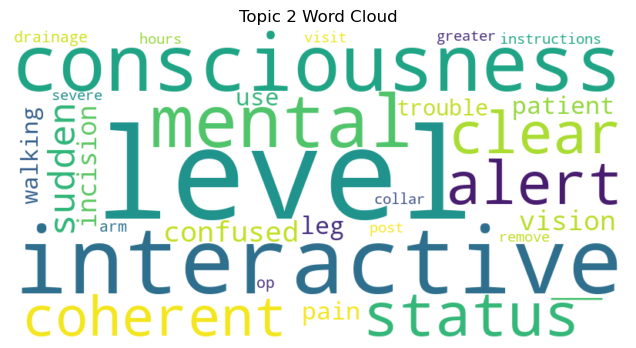
\includegraphics[width=\linewidth]{images/Unsupervised_Results/wordcloud_cluster_1.png}
  \subcaption{This topic cluster consists largely of documents pertaining to the ICF category COM/COG.}
\end{subfigure}
\hfill
\begin{subfigure}{0.45\textwidth}
  \centering
  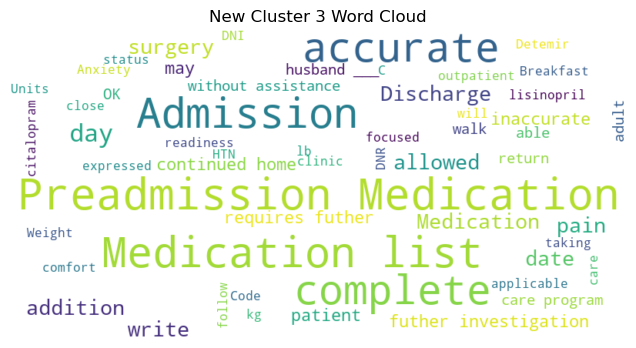
\includegraphics[width=\linewidth]{images/Unsupervised_Results/wordcloud_cluster_3.png}
  \subcaption{This cluster does not appear to contain a dominant semantic theme.}
\end{subfigure}
\caption{Word Clouds for select clusters from K-Means with ClinicalBERT embeddings.}
\label{fig:lda-kmeans-wordclouds-1-3}
\end{figure}

\subsection{Rule-Based with K-Means}

In this approach, a hybrid rule-based system combined with K-Means-based auto-labelling was employed to extract sentences potentially containing functional status information (FSI). The results presented below reflect outcomes from manual inspection and contextual analysis of the labelled outputs.

\begin{table}[H]
\centering
\caption{Manual Inspection of Cluster Labels by ICF Category}
\label{tab:manual-inspection}
\resizebox{\textwidth}{!}{%
\begin{tabular}{lcccc}
\toprule
\textbf{ICF Category} & \textbf{Correct Label (\%)} & \textbf{Contextually Misleading (\%)} & \textbf{Incorrect (\%)} & \textbf{Total Sentences} \\
\midrule
Mobility & 70 & 20 & 10 & 1430 \\[0.5ex]
SCDL & 60 & 30 & 10 & 1149 \\[0.5ex]
IPIR & 30 & 60 & 10 & 870 \\[0.5ex]
COM/COG & 80 & 10 & 10 & 346 \\ 
\bottomrule
\end{tabular}%
}
\end{table}

\begin{figure}[H]
\centering
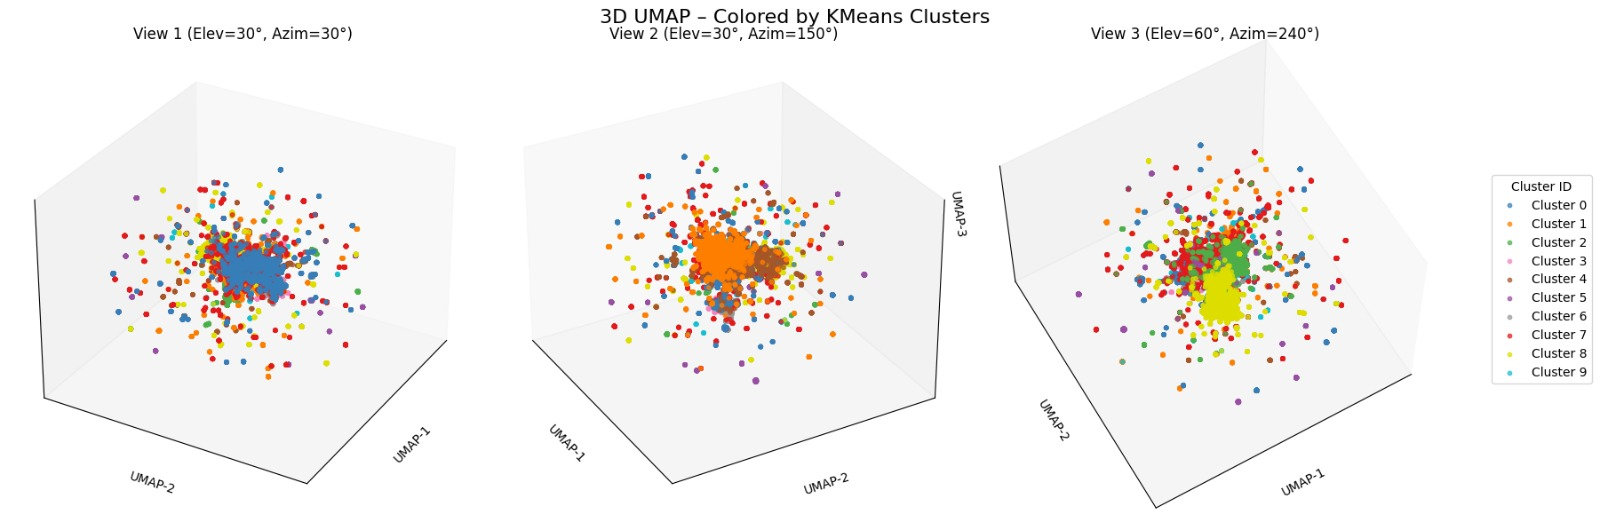
\includegraphics[width=\textwidth]{images/Unsupervised_Results/rulebased_umap_clusters.jpg}
\caption{3D UMAP Visualization of Rule-Based Sentences Colored by K-Means Clusters}
\label{fig:rulebased-kmeans-umap}
\end{figure}

\begin{figure}[H]
\centering
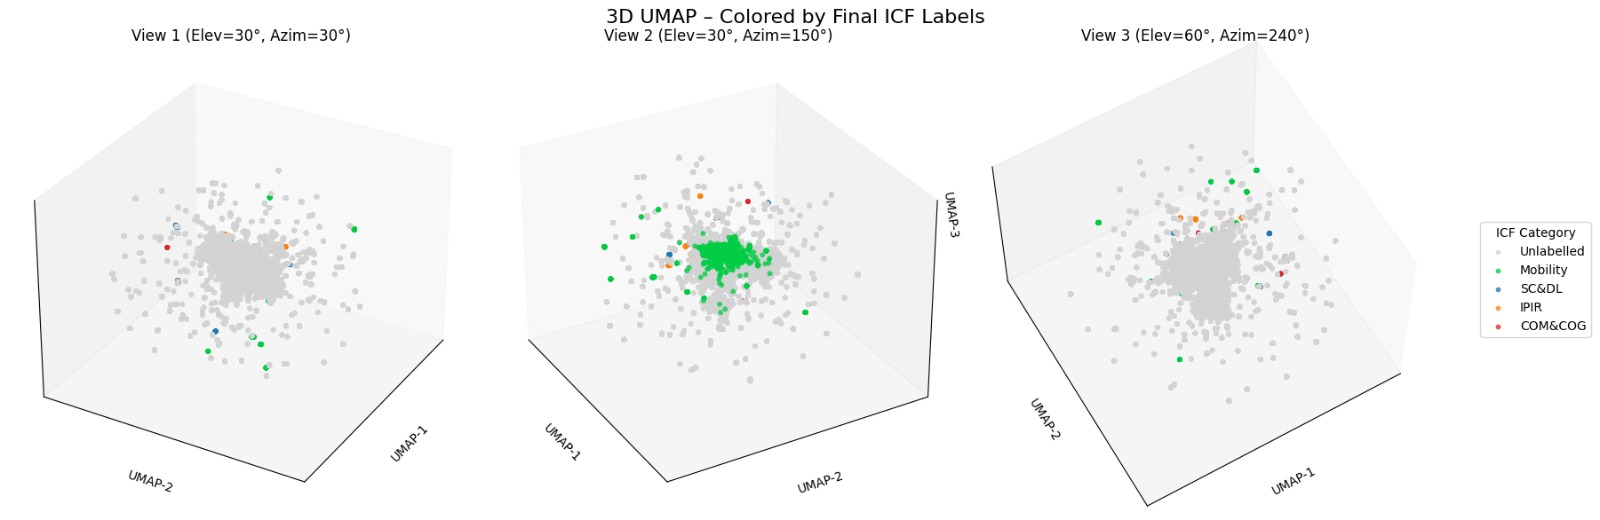
\includegraphics[width=\textwidth]{images/Unsupervised_Results/rulebased_umap_icf_labels.jpg}
\caption{3D UMAP Visualization of Final ICF Domain Labels Assigned to Clusters}
\label{fig:rulebased-umap-icf}
\end{figure}

\begin{figure}[H]
\centering
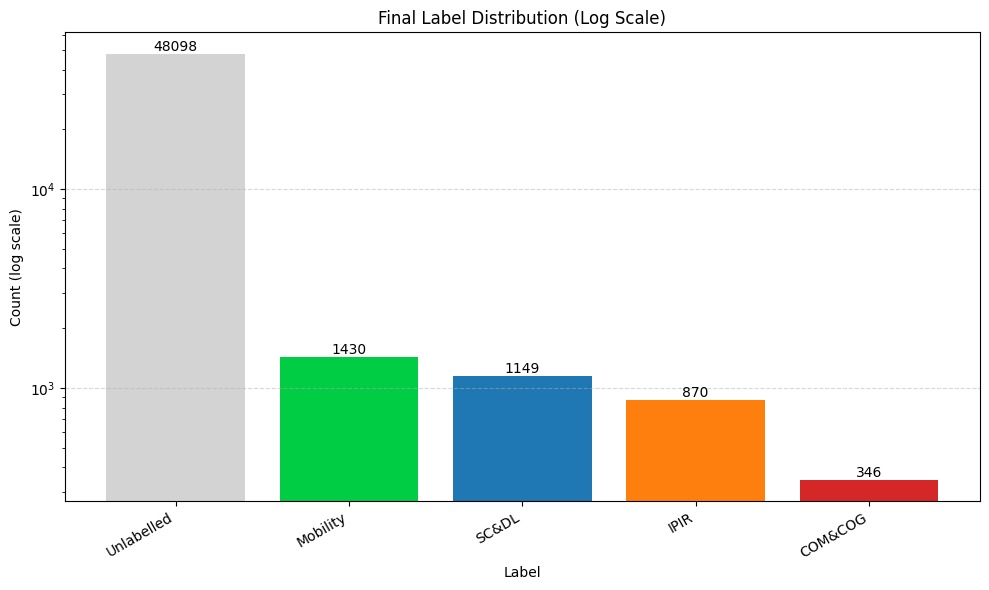
\includegraphics[width=0.65\textwidth]{images/Unsupervised_Results/rulebased_icf_distribution.jpg}
\caption{Final Label Distribution Across ICF Categories (Log Scale)}
\label{fig:rulebased-icf-distribution}
\end{figure}

\vspace{0.5cm}

\begin{table}[H]
\centering
\caption{Precision and Error Summary for Rule-Based with K-Means}
\label{tab:precision-summary}
\begin{tabular}{l c p{8cm}}  % Adjust the width of the last column as needed
\toprule
\textbf{ICF Category} & \textbf{Precision Strength} & \textbf{Main Error Source} \\
\midrule
Mobility & High & Overfitting to generic words like ``run'', ``walk'' \\
SCDL & Moderate & Vague phrases without clear context \\
IPIR & Low & Misclassification on words such as ``family'', ``spouse'' with no interactive context \\
COM/COG & High & Minimal ambiguity \\
\bottomrule
\end{tabular}
\end{table}

\paragraph{Mobility:} Mobility had the highest visibility when it comes to lexical patterns, which explains strong performance. However, overreliance on keywords and phrases, and other surface terms caused conceptual mismatches.

\paragraph{SCDL:} The SCDL dictionary consisted of broad terms which matched some irrelevant medical or procedural language. Semantic embeddings helped slightly, but higher ambiguity remains without sentence-level embeddings.

\paragraph{IPIR:} IPIR suffered heavily due to semantic drift. The term-based approach triggered on certain keywords without ensuring interactional context, which is necessary for a sentence to be classified as IPIR. Hence, clustering amplified this by grouping such mentions and many sentences were wrongly labelled.

\paragraph{Communication and Cognition:} Despite being the category with the lowest number of sentences labelled, COM/COG showed high precision. This is likely due to the well-defined keywords list, which includes words such as \textit{speaking, reading, thinking, etc.}, which co-occur with clinically meaningful context and are picked up well by the model.

\vspace{1em}

\section{Supervised}

\subsection{CNN-RNN}

The CNN-RNN model achieved a micro-F1 score of \textbf{0.7403} and a macro-F1 score of \textbf{0.7294}. Detailed results for each class are presented in Table~\ref{tab:supervised-results}, including the true positives, true negatives, false positives and false negatives for all four domains.

\begin{table}[H]
\centering
\caption{Detailed Classification Results for CNN-RNN Model}
\label{tab:supervised-results}
\begin{tabular}{lccccccc}
\toprule
\textbf{ICF Domain} & \textbf{TN} & \textbf{FP} & \textbf{FN} & \textbf{TP} & \textbf{Precision} & \textbf{Recall} \\ 
\midrule
Mobility & 870 & 45 & 49 & 207 & 0.8214 & 0.8086\\[0.5ex]
Self-care/Domestic Life & 903 & 36 & 74 & 158 & 0.8144 & 0.6810\\[0.5ex]
Interpersonal Interactions & 954 & 49 & 61 & 107 & 0.6859 & 0.6369\\[0.5ex]
Communication/Cognition & 965 & 34 & 61 & 111 & 0.7655 & 0.6453\\ 
\bottomrule
\end{tabular}
\end{table}

Note that sentences not labeled with any of the four ICF categories were assigned a label of 0 and included in the ‘full dataset’ to reflect real-world class imbalance.

\begin{figure}[H]
\centering
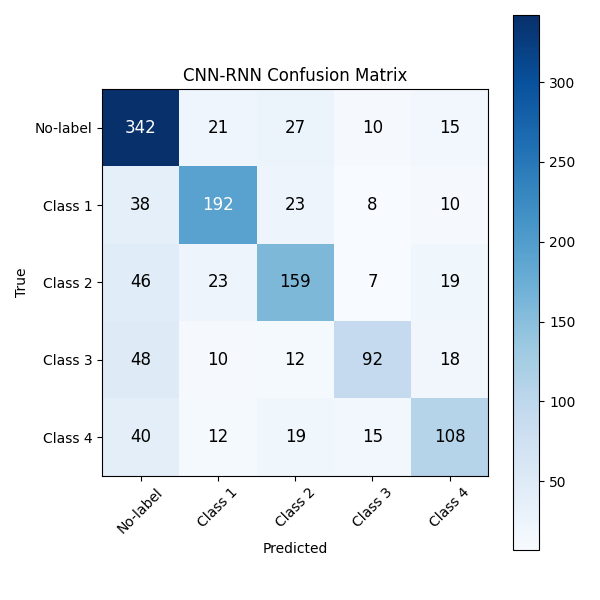
\includegraphics[width=0.6\textwidth]{images/Supervised_Results/cnn-rnn_confusion_matrix.png}
\caption{Confusion Matrix for the CNN-RNN Model}
\label{fig:cnn-rnn-confusion-matrix}
\end{figure}

As shown in Fig. \ref{fig:cnn-rnn-confusion-matrix}, the CNN-RNN model achieves strong classification for Mobility but struggles slightly with IPIR, evidenced by higher false negatives.

\begin{figure}[H]
\centering
\begin{minipage}[b]{0.48\textwidth}
    \centering
    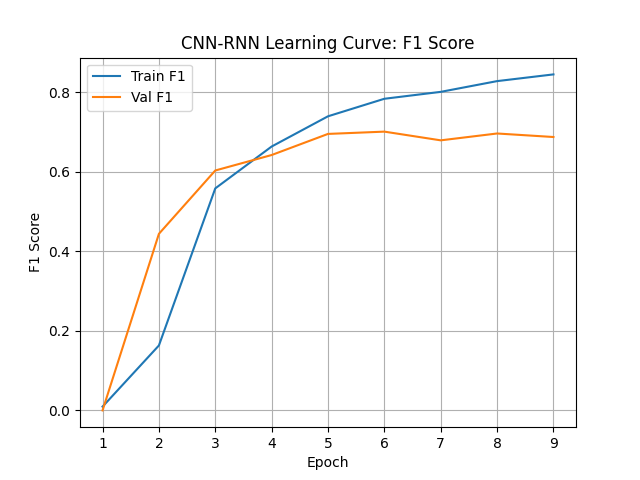
\includegraphics[width=\textwidth]{images/Supervised_Results/cnn-rnn_learning_curve_f1.png}
    \caption{Learning Curve (F1-Score) for the CNN-RNN Model}
    \label{fig:cnn-rnn-learning-curve-f1}
\end{minipage}
\hfill
\begin{minipage}[b]{0.48\textwidth}
    \centering
    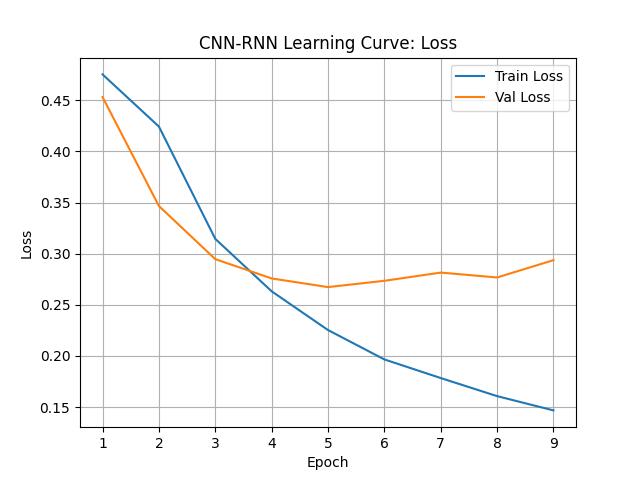
\includegraphics[width=\textwidth]{images/Supervised_Results/cnn-rnn_learning_curve_loss.png}
    \caption{Learning Curve (Loss) for the CNN-RNN Model}
    \label{fig:cnn-rnn-learning-curve-loss}
\end{minipage}
\end{figure}

Fig. \ref{fig:cnn-rnn-learning-curve-f1} and Fig. \ref{fig:cnn-rnn-learning-curve-loss} show the learning curves for the CNN-RNN hybrid model, these curves show the training and validation F1 Score and loss over nine epochs, since early stopping was triggered.

\vspace{1em} 
\subsection{FNN}

The FNN model reached a micro-F1 score of \textbf{0.6713} and macro-F1 score of \textbf{0.6611}. Detailed results for each class are presented in Table~\ref{tab:fnn-results}, including the true positives, true negatives, false positives and false negatives for all four domains.

\begin{table}[H]
\centering
\caption{Detailed Classification Results for FNN Model}
\label{tab:fnn-results}
\begin{tabular}{lccccccc}
\toprule
\textbf{ICF Domain} & \textbf{TN} & \textbf{FP} & \textbf{FN} & \textbf{TP} & \textbf{Precision} & \textbf{Recall} \\ 
\midrule
Mobility & 854 & 61 & 75 & 181 & 0.7479 & 0.7070 \\
Self-care/Domestic Life & 872 & 67 & 76 & 156 & 0.6996 & 0.6724 \\
Interpersonal Interactions & 952 & 51 & 71 & 97 & 0.6554 & 0.5774 \\
Communication/Cognition & 963 & 36 & 79 & 93 & 0.7209 & 0.5407 \\
\bottomrule
\end{tabular}
\end{table}

\begin{figure}[H]
\centering
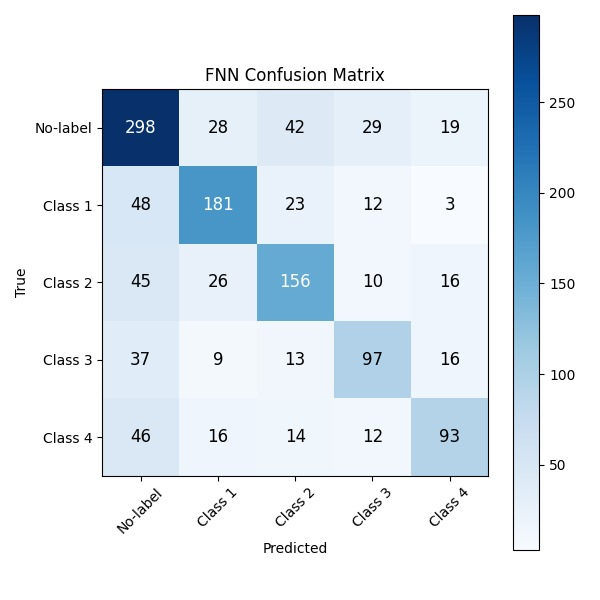
\includegraphics[width=0.6\textwidth]{images/Supervised_Results/FNN_confusion_matrix.jpg}
\caption{Confusion Matrix for the FNN Model}
\label{fig:fnn-confusion}
\end{figure}

As shown in Fig. \ref{fig:fnn-confusion}, like the CNN-RNN model, the FNN model achieves strong classification for Mobility but struggles slightly with IPIR, evidenced by higher false negatives.

\begin{figure}[H]
\centering
\begin{minipage}[b]{0.48\textwidth}
    \centering
    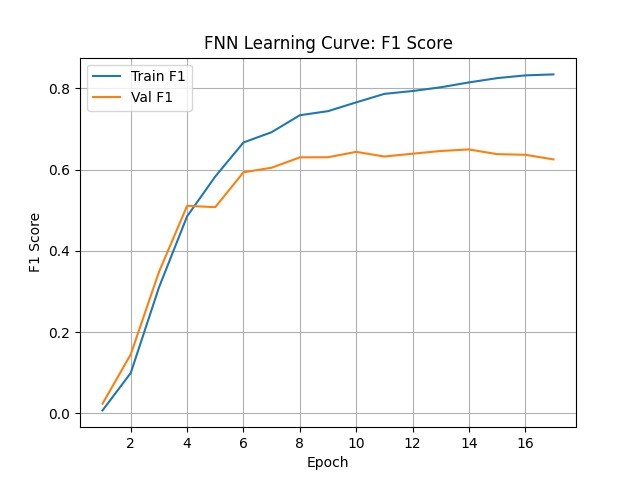
\includegraphics[width=\textwidth]{images/Supervised_Results/FNN_learningcurve_F1score.jpg}
    \caption{F1 Score Learning Curve - FNN}
    \label{fig:fnn-f1}
\end{minipage}
\hfill
\begin{minipage}[b]{0.48\textwidth}
    \centering
    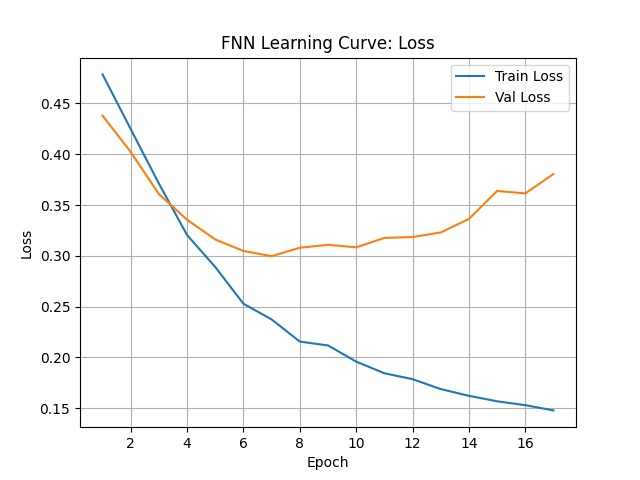
\includegraphics[width=\textwidth]{images/Supervised_Results/FNN_learning_curve_loss.jpg}
    \caption{Loss Learning Curve - FNN}
    \label{fig:fnn-loss}
\end{minipage}
\end{figure}

Fig. \ref{fig:fnn-f1} and Fig. \ref{fig:fnn-loss} show the learning curves for the FNN model, these curves show the training and validation F1 Score and loss over sixteen epochs, since early stopping was triggered.

\subsection*{Additional Models Considered}

In addition to the CNN-RNN and FNN models, a Random Forest classifier was also used. However, due to its underperformance and lack of generalizability, we omit detailed results for the Random Forest model. % Mahesh 1000
% Tara - Discussion and conclusions — This section should include a critical discussion of your findings, which relates them to the wider body of knowledge that you described in the literature review.
% You should cover the significance of your results, any limitations to your approach, and outline next steps for future research. This section should culminate in your conclusions, which should link back to the research question and objectives.

\chapter{Discussion and Conclusion}

\section{Motivation and Context}

The primary motivation behind this study was to explore how different techniques in natural language processing (NLP) — including both, supervised and unsupervised learning — can enable the extraction of Functional Status Information (FSI) from free-text clinical records, particularly in the absence of a publicly available, high-quality gold-standard dataset. The challenges inherent in this task are considerable: FSI is sparsely expressed, context-dependent, and frequently implicit in clinical text. Yet capturing this information is critical for patient-centred care and may be used for outcome prediction, as highlighted in the literature \cite{newman2019broadening}. Our project, therefore, sought to evaluate how existing methods from the NLP and health informatics literature could be applied to FSI classification across the four different ICF domains.

\section{Unsupervised Approaches: Significance of Results}

Unsupervised learning played a foundational role in exploring thematic structures within discharge summaries from the MIMIC-IV dataset. In the absence of reliable labels, models such as LDA and K-Means clustering were used to uncover latent semantic groupings. \medskip

The \textbf{LDA with Term-Frequency and K-Means with ClinicalBERT embedding} clusters revealed that meaningful topic separation is feasible as an initial step in identifying topics within this high volume unlabelled data. Silhouette scores for the K-means model stabilised around 0.72 for four- and five-topic models. These results suggest the presence of underlying structure in FSI-related sentences, in line with earlier findings in thematic modelling of medical narratives \cite{low2020nlp}. 
Perhaps owing to the bag-of-words representation, LDA clusters could not capture deeper contextual meanings required for nuanced functional classification.
\medskip

In contrast, \textbf{K-Means clustering with ClinicalBERT embeddings} provided more

semantically meaningful groupings for two of the categories. For example, in the
Communication and Cognition domain, 80\% of the manually inspected labels matched the cluster-assigned label, and in Mobility, this figure was 70\%. Sentences pertaining to more abstract domains such as Interpersonal Interactions and Self-care/Domestic Life were not notably grouped together in clusters, pointing to the limits of unsupervised methods in performance across the categories.
\medskip

The unsupervised pipeline offers a \textbf{valuable early-stage framework} for segregating the large dataset into meaningful groups, particularly in low-resource settings. It is significant that such a method could yield a relatively robust performance in some domains - it can minimize the need for manual supervision and analysis of discharge summaries. Valuable insights emerged from the clustering approaches which may be applicable for the development of initial training datasets for downstream NLP tasks—for instance, identifying which ICF categories may require more nuanced handling during annotation efforts. 

\section{Supervised Approaches: Significance of Results}

Supervised learning, supported by a manually annotated silver-standard dataset, formed the second core methodology investigated in the project. Three models were evaluated: a CNN-RNN hybrid, a Feedforward Neural Network (FNN), and a Random Forest classifier.
\medskip

A hybrid \textbf{CNN-RNN model} achieved the highest overall performance when considering the evaluation with a micro-F1 score of 0.74 and macro-F1 of 0.73. This is attributed to the possibility that a recurrent structure enabled it to capture sequential and syntactic nuances in clinical sentences. The ICF category labels were predicted with intriguingly high precision (0.82), recall (0.81) and F1 scores. These findings are encouraging and suggest that further investigation into the application of these techniques for functional status information extraction is both justified and warranted. Nonetheless, these results must be interpreted with some caution due to the absence of high-quality ground truth labeled data.
\medskip

The \textbf{FNN}, although simpler, achieved a respectable micro-F1 of 0.67. This model's lower complexity and faster training time make it suitable for environments with limited computational resources, despite its inability to model complex sentence structures. 
\medskip

The \textbf{Random Forest classifier}, leveraging a hybrid feature set of TF-IDF and FastText embeddings, exhibited comparatively lower performance, underscoring the potential advantages of employing more advanced NLP techniques in this domain.
\medskip

The significance of these results lies in their demonstration that supervised learning is feasible for multi-label classification of FSI even with modestly sized and imperfectly annotated training data. The supervised classification models further confirm that despite annotation challenges, supervised pipelines can operationalise ICF-based classification in a scalable manner.

\section{Limitations}

Despite promising results, this project is constrained by several notable limitations:

\subsection{Annotation Quality}

The most critical limitation was \textbf{the quality and consistency of the annotated dataset}. Albeit considerable effort was made to manually annotate a representative sample of sentences, a high percentage of annotations were later found to be inconsistent or ambiguous upon cross-validation. The absence of medically trained annotators and the subjective nature of functional status language further undermines the reliability of the dataset. This annotation noise had a twofold impact: the compromised annotation quality not only impacted the reliability of supervised model training but also precluded the use of conventional classification metrics—such as accuracy—for evaluating unsupervised outputs. To uphold methodological rigor, evaluation was instead conducted using perplexity and silhouette scores, complemented by systematic manual error analysis.

\subsection{Evaluation Metrics for Unsupervised Learning}

Due to the absence of trustworthy ground truth labels for the majority of the corpus, unsupervised methods were evaluated using perplexity and silhouette scores. While these metrics are valid for assessing intra-cluster cohesion and topic coherence, they do not reflect classification accuracy. Accordingly, the evaluation of clustering methods remains inherently indirect and highlights the need for validation against expert-annotated benchmark datasets in future research.

\subsection{Domain and Data Coverage}

The dataset was restricted to four ICF domains and our models were trained solely on ICU discharge summaries from a U.S.-based institution, which may limit generalizability to other clinical contexts, such as primary care or the NHS in the UK.

\section{Topics for Future Research}

This project opens up several important avenues for future research that align closely with the original research questions and objectives.

\subsection{Development of a Gold-Standard Dataset}

Future work must prioritise the creation of a gold-standard annotated corpus, developed in close collaboration with domain experts. Annotation guidelines provide a solid foundation, need to be complemented with multiple rounds of feedback and inter-annotator agreement analysis. A high-quality, publicly available gold dataset would not only enable rigorous technological advancement but also catalyse further research in this space.

\subsection{Improving Annotation Workflows}

To address the challenge of annotation burden, semi-supervised approaches like active learning can be used to identify high-value sentences for manual review. With the time constraints, it was not possible to implement an active learning technique as set out in  Le et al.’s 2023 paper \cite{le2023}, though this would have provided a more accurately labelled dataset. It is a complicated technique that is unfamiliar to the group, so it would take a long time to implement and still requires domain experts to achieve an actual gold-standard labelled dataset. Another solution to fix the problem of having no annotated dataset would be to have employed Newman-Griffis and Fosler-Lussier’s method \cite{newman-griffis2020auto} of using a weakly supervised model based on the ICF guidelines rather than having to create a labelled dataset, though the F1-Score achieved using this method was similar to our best model’s performance.

\subsection{Longitudinal Modelling of Functional Status}

The current work treats each sentence in isolation. However, functional status is inherently temporal and contextual. Future models could integrate longitudinal data from EHRs—such as change over time or response to treatment—using time-aware models or graph neural networks. This would enable more dynamic and predictive FSI extraction pipelines.

\subsection{Interpretability and Clinical Utility}

To ensure real-world adoption, future models may wish to ensure interpretability. Interpretability of technical models is essential for real-world adoption because it builds clinician trust and supports accountability and an understanding of why models are effective. Doctors are more likely to embrace NLP-based applications if they can see why it makes a classification and what might lead to errors, which can in turn satisfy regulatory expectations for transparency and reliability.

\section{Conclusion}

This project has demonstrated that functional status information—though sparse and contextually complex—can be extracted from free-text clinical notes using a combination of supervised and unsupervised learning techniques in natural language processing. Our unsupervised pipeline provided valuable thematic insights and a mechanism for scalable early-stage labeling, while our supervised models validate the hypothesis that even noisy, silver-standard annotations can support effective multi-label classification in this context.
\medskip
These findings directly address the core research questions the team sought to investigate, confirming that both approaches are viable for early-stage FSI extraction from discharge summaries and its classification. Both techniques have much to offer to organizations and researchers interested in its analyses and in leading annotation efforts. That being said, current limitations in annotation quality and domain coverage necessitate caution in the interpretation of performance evaluations and underscore the need for continued and methodological development of the application of these techniques.\medskip

Ultimately, this work contributes to a growing body of literature that seeks to bridge the gap between narrative clinical documents and structured, actionable data—an endeavour that is crucial for enabling advanced patient-centred care and clinical decision support in healthcare systems of the future. % Tara Discussion and Conclusion 1500 - 2000
\bibliographystyle{IEEEtran}
\bibliography{mybibliography}
\end{document}

% Roughly 9000 - 10000 range total.